\chapter[Introduction]{Introduction}
\label{cha:Chapter1}
\vspace*{\fill}


\newpage

\section{Background}


\subsection{Land cover}

    Land cover---the physical and biological material found on the surface of the earth---encompasses natural environments like forests, grasslands, wetlands, and things made by humans, like urban areas, croplands, and infrastructure. 
    
    Its study and monitoring are crucial for a multitude of reasons. Land cover changes significantly influence regional and global climate patterns and are a major driver of biodiversity loss, emphasizing the necessity of monitoring for climate change mitigation and biodiversity preservation \citep{pielke2002influence, houghton2012carbon, sala2000global, cbd2016indicators}. 
    
    Additionally, these changes have direct implications for the quality and availability of natural resources, such as water and air \citep{foley2005global}. Land cover assessment is vital for evaluating the livability of human environments \citep{krekel2016greener,levering2024landscape} and has key applications in informing policy, analyzing land-based emissions, and estimating local climate extremes \citep{duveiller2020, hong2021luemissions, sy2020,}. 

    Therefore, understanding land cover dynamics is crucial for effective policy-making at both regional and global levels \citep{liu2020assessing, trisurat2019land, shumba2020effectiveness}. As different entities with different objectives require maps with different things on them, the choice of which type of land cover to map is a central one. 

\subsection{General land cover classes}

    \subsubsection{Crops and Grasslands}

        Croplands and grasslands are essential for food production, and together cover over 40\% of the European Union's territory \citep{eurostat2021land}. European cropland is a diverse land cover type; over 100 crops are produced at scale in Europe, ranging from cereals such as wheat and rice to sunflowers, tobacco, and herbs such as basil and valerian \citep{eurostat2023agricultural}. Grasslands, on the other hand, cover wide roles beyond dairy and meat production: water supply and flow regulation, carbon storage, erosion control, climate mitigation, pollination, and cultural significance \citep{bengtsson2019grasslands}. 
        
        The agricultural sector is not only a cornerstone of the EU's economy, but also a significant employer, with approximately 4.2\% of the EU's population engaged in agriculture. Reflecting its importance, the European Union's Common Agricultural Policy (CAP) has earmarked {\texteuro}264 billion as agricultural subsidy for the 2023--2027 period. The economic magnitude of crop and livestock production makes tracking and understanding their dynamics in the EU a priority for many stakeholders.

    \subsubsection{Forests}

        Forests cover nearly a third of the planet's land area \citep{fao2022,banskota2014forest} and more than 41\% of the EU \citep{eurostat2021land}. They are important for biodiversity \citep{cazzolla2022number}, carbon sequestration \citep{ipcc2021}, and have been supplying a plethora of resources used by human civilization since the palaeolithic. Given recent trends of globalization and deforestation, monitoring forest cover change and its drivers is crucial \citep{sy2019tropical,masolele2024mapping} for a great number of actors, including the UN and national governments, the industrial sector, local communities, and Indigenous peoples.

        National forest inventories, statisticians, and mapping organizations often disagree about the quantity of forest in any given area, which can lead to fierce scientific debates \citep{picard2021recent, korhonen2020new, palahi2021concerns, rossi2019assessing}
    
    \subsubsection{Wetlands}

        Wetlands, recognized as one of the most biologically productive and important natural ecosystems, play a pivotal role in regulating the global climate, maintaining the hydrological cycle, and supporting diverse species \citep{hu2017global,ramsar2001wetlands}. The unique hydrology of these ecosystems influences the distribution of sediment, nutrients, flora, and fauna. They provide essential services such as improving water quality, flood mitigation, recharging aquifers, and supporting an array of wildlife \citep{costanza1997value,smardon2009sustaining}. Despite these benefits, wetlands have historically been undervalued, often seen as wastelands or disease sources, leading to significant losses due to reclamation and degradation \citep{giblett1996postmodern,owens2001global,davidson2014much,gardner2018global,dugan1993wetlands,oecd1996guidelines,ramsar2015wetlands}. The world has witnessed a dramatic decline in wetland areas, with an estimated 87\% degradation since 1700, particularly in the 20th and early 21st centuries, resulting in substantial economic losses and reduced ecosystem service value \citep{gardner2015state,costanza2014changes}. While they only cover 1.7\% of the EU \citep{eurostat2021land}, their vital role and the alarming rate of loss make it crucial to preserve their ecological integrity and ensure the continued provision of their invaluable ecosystem services.

    \subsubsection{Land Use}

        There is another way besides land \textit{cover} to describe land: With land \textit{use}. Land Use does not refer to what's there, but how it is being used by humans. A grassland can be an intensively grazed pasture or a protected nature reserve. A 'forest' can be a palm oil plantation, a recreational area, or a rare old-growth forest with religious significance. The term 'Land Use' is sometimes used interchangeably with Land Cover \citep{fisher2005land}, and different authors make different distinctions. For example, \citet{hansen2022global} group inland water and wetlands as land cover, and built-up area, cropland and tree cover change as land use. Sometimes, a legend contains classes that are combinations of Land Use / Land Cover (LULC), such as pastures and natural grasslands in CORINE land cover, or even the grass fields at airports in the LUISA Basemap of Europe \citep{pigaiani2021luisa}. Because such classes can be ambiguous and hard to map by computer programs, they are not often reproduced at scale with remote sensing techniques. The LUCAS survey makes a clear distinction between land use and land cover: each observation has a separate listing for both types, with some combinations occurring frequently (like \textit{agricultural} use and \textit{grassland} cover to represent \textit{pastures}), and others being extremely rare (\textit{residential} use and \textit{peat bog} cover).

    \subsubsection{What should be on a map?}

        Broad categories such as 'Forest' or 'Water' are relatively simple for people and computers to differentiate. However, adding more detail to the map by splitting up these big categories into more specific classes, or improving the \textit{thematic resolution}, brings many challenges. 
        
        First of all, maps with many classes are hard to read by humans. Reading a complex map is not always necessary, as users can derive simpler maps from rich datasets to tailor them to their use case \citep{tsendbazar2017integrating} or use the mapped values for a different type of analysis. 

        Secondly, the process of making detailed maps is more costly and difficult. You need to collect more examples from more different categories, and not all categories are equally easy to distinguish by surveyors. Someone interpreting aerial imagery might be able to distinguish grassland from forest, but what if they want to map different tree species, or distinguish pastures from natural grassland?

        Which brings us to the next question: How do you get those maps in spite of those challenges? People used to draw maps based on field surveys. Later maps were based on aerial imagery. In recent decades, we have been increasingly using remote sensing and machine learning.

                

        \subsubsection{Land cover and land use mapping and monitoring in EU}

        Especially in Europe, long-running datasets, such as CORINE land cover and the LUCAS survey \citep{lucas,dandrimont2021lucas}, have provided detailed and consistent land cover information for almost two decades \citep{gallego2008using}. 
        
        A good example of a detailed land cover dataset experiencing this transition is the CORINE (Coordination of Information on the Environment) Land Cover Project. CORINE is an initiative by the European Environment Agency (EEA) that aims to collect information on the land cover of Europe to support environmental policy development. The project started in 1985 as part of the European Commission’s CORINE program, designed to gather and harmonize data related to the environment across the member states. In the subsequent decades, it was used to assess land cover changes in Europe \citep{mucher2000land, feranec2010determining}. 

        However, as the project evolved and standards for environmental data became more stringent, its limitations became increasingly apparent. 
        The nature of its legend, which often combines land use and land cover within the same category, and the presence of mixed classes such as \emph{``airport''} (grass, buildings, roads)
        Furthermore, the project's reliance on a 25 hectare minimum mapping unit for most LULC types means that it only contains relatively large patches (see Fig\@~\ref{fig:biesbosch_osm_clc}). This means it underrepresents LULC types and is of limited accuracy at fine spatial scales \citep{buttner2014corine,aune2021content, pflugmacher2019mapping}. Regardless, CLC is among the most popular and widely used European land cover datasets, and should not be discarded. As using human cartographers at a finer spatial and temporal scale would be prohibitively difficult, slow, and costly, attempts have been made to automate the production of CLC \citep{buttner2014corine}, but usually at a lower thematic resolution, for example for 12 \citep{pflugmacher2019mapping} or 14 \citep{bhugra2022rapidai4eo} classes. There have also been other projects that accurately map European land cover at high spatial resolution using different legends that are more optimized for a remote sensing context, such as S2GLC \citep{malinowski2020}, and attempts to specifically map crop types with specialized approaches \citep{dandrimont2021parcel,luo2022developing}
        
        \begin{figure}[H]
        \centering
    
        % First row with two subfigures side by side
        \begin{subfigure}[b]{0.48\textwidth}
            \centering
            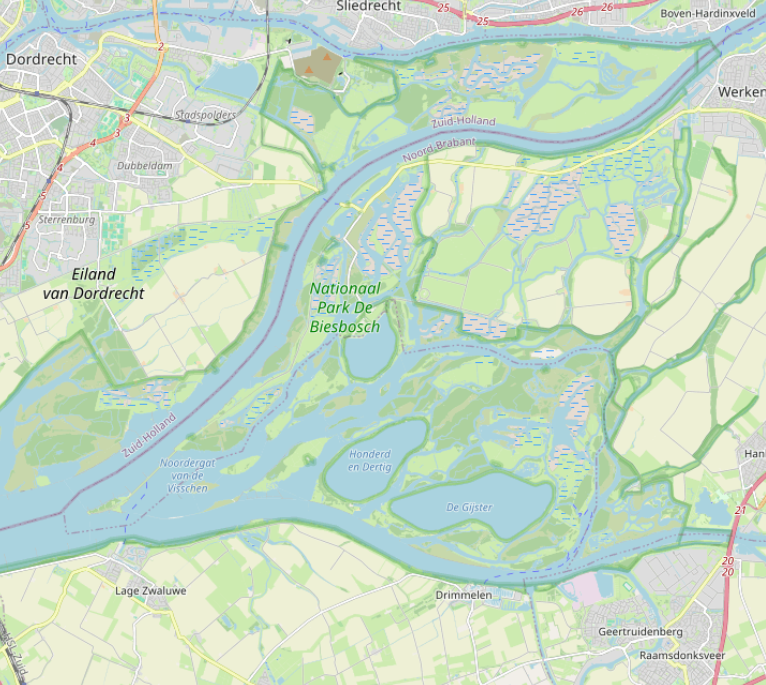
\includegraphics[width=1\linewidth,height=\linewidth]{figs_01/biesbosch_osm.png}
            \caption{OpenStreetMap}
            \label{fig:biesbosch_osm}
        \end{subfigure}
        \hfill % Space between the first two subfigures
        \begin{subfigure}[b]{0.48\textwidth}
            \centering
            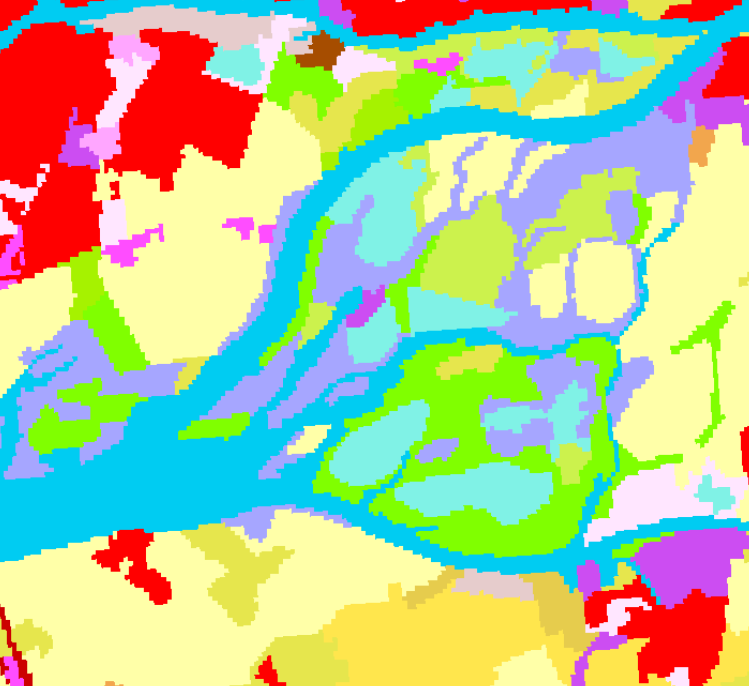
\includegraphics[width=1\linewidth,height=\linewidth]{figs_01/biesbosch_clc.png}
            \caption{Corine Land Cover}
            \label{fig:biesbosch_clc}
        \end{subfigure}
        \caption{Representation of the Biesbosch wetlands area in the Netherlands in OpenStreetMap and Corine Land Cover 2018}
        \label{fig:biesbosch_osm_clc} % This should be inside the figure environment but outside any subfigure
        \end{figure}

\subsection{Land cover classification with machine learning and earth observation data}
    
    Automated mapping methods, such as those used by \citet{pflugmacher2019mapping}, \citet{dandrimont2021parcel}, \citet{luo2022developing} and \citet{malinowski2020automated} are called Land Cover Classification. It typically involves showing many good examples of the things you want to detect on a map to a computer program, which then learns how to recognize them by itself when shown new locations. For this, the following three core components are needed:
    
    \begin{itemize}
        \item \textbf{Examples:} Confirmed observations of different types of land cover, with a known time and place. We call this \textbf{reference data}.
        \item \textbf{Earth observation (EO) data:} satellite imagery and other geographic data that cover the area you want to map. Together, these \textbf{covariates} form the \textbf{feature space}. Spatial and temporal metadata allow aspiring mappers to combine several existing, unrelated datasets into one feature space; a rarity in the machine learning domain.
        \item A \textbf{model:} Some kind of decision-making algorithm that learns to recognize which examples often occur at which combination of the covariates. If this goes well, you can use it to \textbf{predict} which land cover occurs at locations where you don't have reference data, but which are covered by the feature space \citep{meyer2021predicting}.
    \end{itemize}
    
    It is common to use different sets of reference data: one set to train your model, and one independent set to validate its predictions, namely the land cover maps it has made. It is good if these two datasets were collected separately from each other, because this helps to make sure your model \textbf{generalizes} well: that its predictions are accurate in new situations, not just on the data it was trained on.

    \subsubsection{Training data}

        Training data is a set of labeled observations that are used to teach a machine learning model to recognize similar things in new situations. 
        
        The goal of most trained models is that they \textbf{generalize} well, which means that they can make consistent and accurate estimations in areas and moments they were not trained on. To make sure your model generalizes well, you have to properly represent the feature space of the area you want to map in your training data \citep{meyer2021predicting}. This does not directly relate to geographical space; large homogeneous areas such as deserts tend to be quite similar in the feature space, while small complex landscapes such as cities with parks, gardens and canals will show great local variation. 

        It is important to have enough training examples \citep{ramezan2021effects,rodriguez-perez2017influence,zhu2016optimizing}, but what is `enough' differs per model \citep{myburgh2014impact} and task \citep{koshute2021recommending}.
        
        Models often learn to estimate classes in the same proportions as their training data. If these proportions do not match the real-world situation of the area they need to map, the model is \textbf{biased}. To minimize this bias and predict the right relative quantities for each class, you need training data that match the desired proportions \citep{he2009learning, kleinewillinghofer2022unbiased}.
        
    \subsubsection{Validation data}

        All maps are wrong \citep{monmonier2018how}, and maps produced with machine learning and earth observation data are no exception. Errors can be defined as \textit{quantity disagreement} and \textit{allocation disagreement}: are there enough pixels of every class, and are they in the right place \citep{pontius2006can,pontius2011death}? Ideally, both types of errors should be low. Errors can come from various sources. Some classes might be hard to distinguish in the available feature space, confusing the model \citep{shivakumar2017spectral}. Some classes might be overrepresented in the training data, leading the model to predict it more frequently at the expense of other classes and resulting in low quantity agreement.

        In general, it is essential that any map is validated with a set of observations. Such validation datasets need to be of high quality: their accuracy should surpass the target accuracy of the map and they need to be representative of the classes in the mapped area.
    
        Biased training data can lead to a biased model that overpredicts certain classes. In this case, the proportions of the classes on the map will deviate from the proportions in the real world. It is very difficult to quantify the bias of a model before it is used \citep{stehman2013estimating}, and the current best way of fixing the proportions on a map is to measure the model bias with additional sampling after the mapping is complete \citep{stehman2014estimating}.

        Classification errors become even more troublesome when land cover change is measured by comparing maps from two time periods, as any misclassified pixel will be interpreted as a change \citep{olofsson2013making}. This can be counteracted by careful sampling design \citep{stehman2012impact,olofsson2014good}, although some work has been done to circumvent this and derive area estimates directly from the model predictions \citep{sales2022land,kleinewillinghofer2022unbiased,angelopoulos2023predictionpowered}.

    \subsubsection{Earth Observation Data}

        Earth observation data refers to measurements taken by sensors at various ranges, from ground measurements \citep{shahi2015novel} to drone \citep{tang2015precise} and airplane \citep{mastelic2020aerial} imagery, to satellite scans \citep{phiri2020sentinel}. The most useful for recurring large-scale mapping are satellite scans, as satellites revisit the same area at a regular pace. This allows them to provide a consistent stream of data, which, in some cases, can continue for decades \citep{xiong2020modis,wulder2022fifty}.

        Earth observation data only started becoming openly available after Brazil published its LANDSAT archives as open data in 2008 \citep{nature2008markets}. Afterwards, more and more Earth observation data and land cover information has become openly available. 
    
        While this rapidly growing landscape of increasingly large datasets on diverging platforms and systems can be hard to navigate \citep{wagemann2021a}, it has fuelled an exponential increase in the amount of mapping initiatives and environmental awareness \citep{wulder2022fifty}, with applications ranging from deforestation \citep{hansen2013high} to soil mapping \citep{hengl2017soilgrids250m}.
        
        Spatial machine learning is unique in the sense that it allows modelers to easily combine variables if they can somehow acquire a representation of them at the time and place of the ground truth observation, such as with a spatial or spatiotemporal overlay. Combining different data sources can lead to much higher performance, for instance with crop stress detection  \citep{berger2022multi}, urban heat \citep{shahi2015novel}, and land cover classification \citep{zhu2016optimizing, hurskainen2019auxiliary, hosseiny2022urban}. Having data of the same place from different moments \citep{low2013impact} and different spatial resolutions or scales \citep{santos2012multiscale} can also improve mapping accuracy, especially of classes that have very similar spectral profiles and/or cyclical temporal dynamics, such as crops and grassland \citep{esch2014differentiation}.

% \subsection{Land cover and land use classification systems}

% Unfortunately, the number of land cover / land use classification systems is often as large as the number of products. On the positive side, many systems are in fact compatible and are using somewhat different words for practically the same ontology. Currently the most used LULC classifications systems include:

% \begin{itemize}
%     \item GLC-CCI (global)
%     \item CORINE (Europe)
%     \item EAGLE (Europe)
% \end{itemize}

% \begin{figure}
%     \centering
%     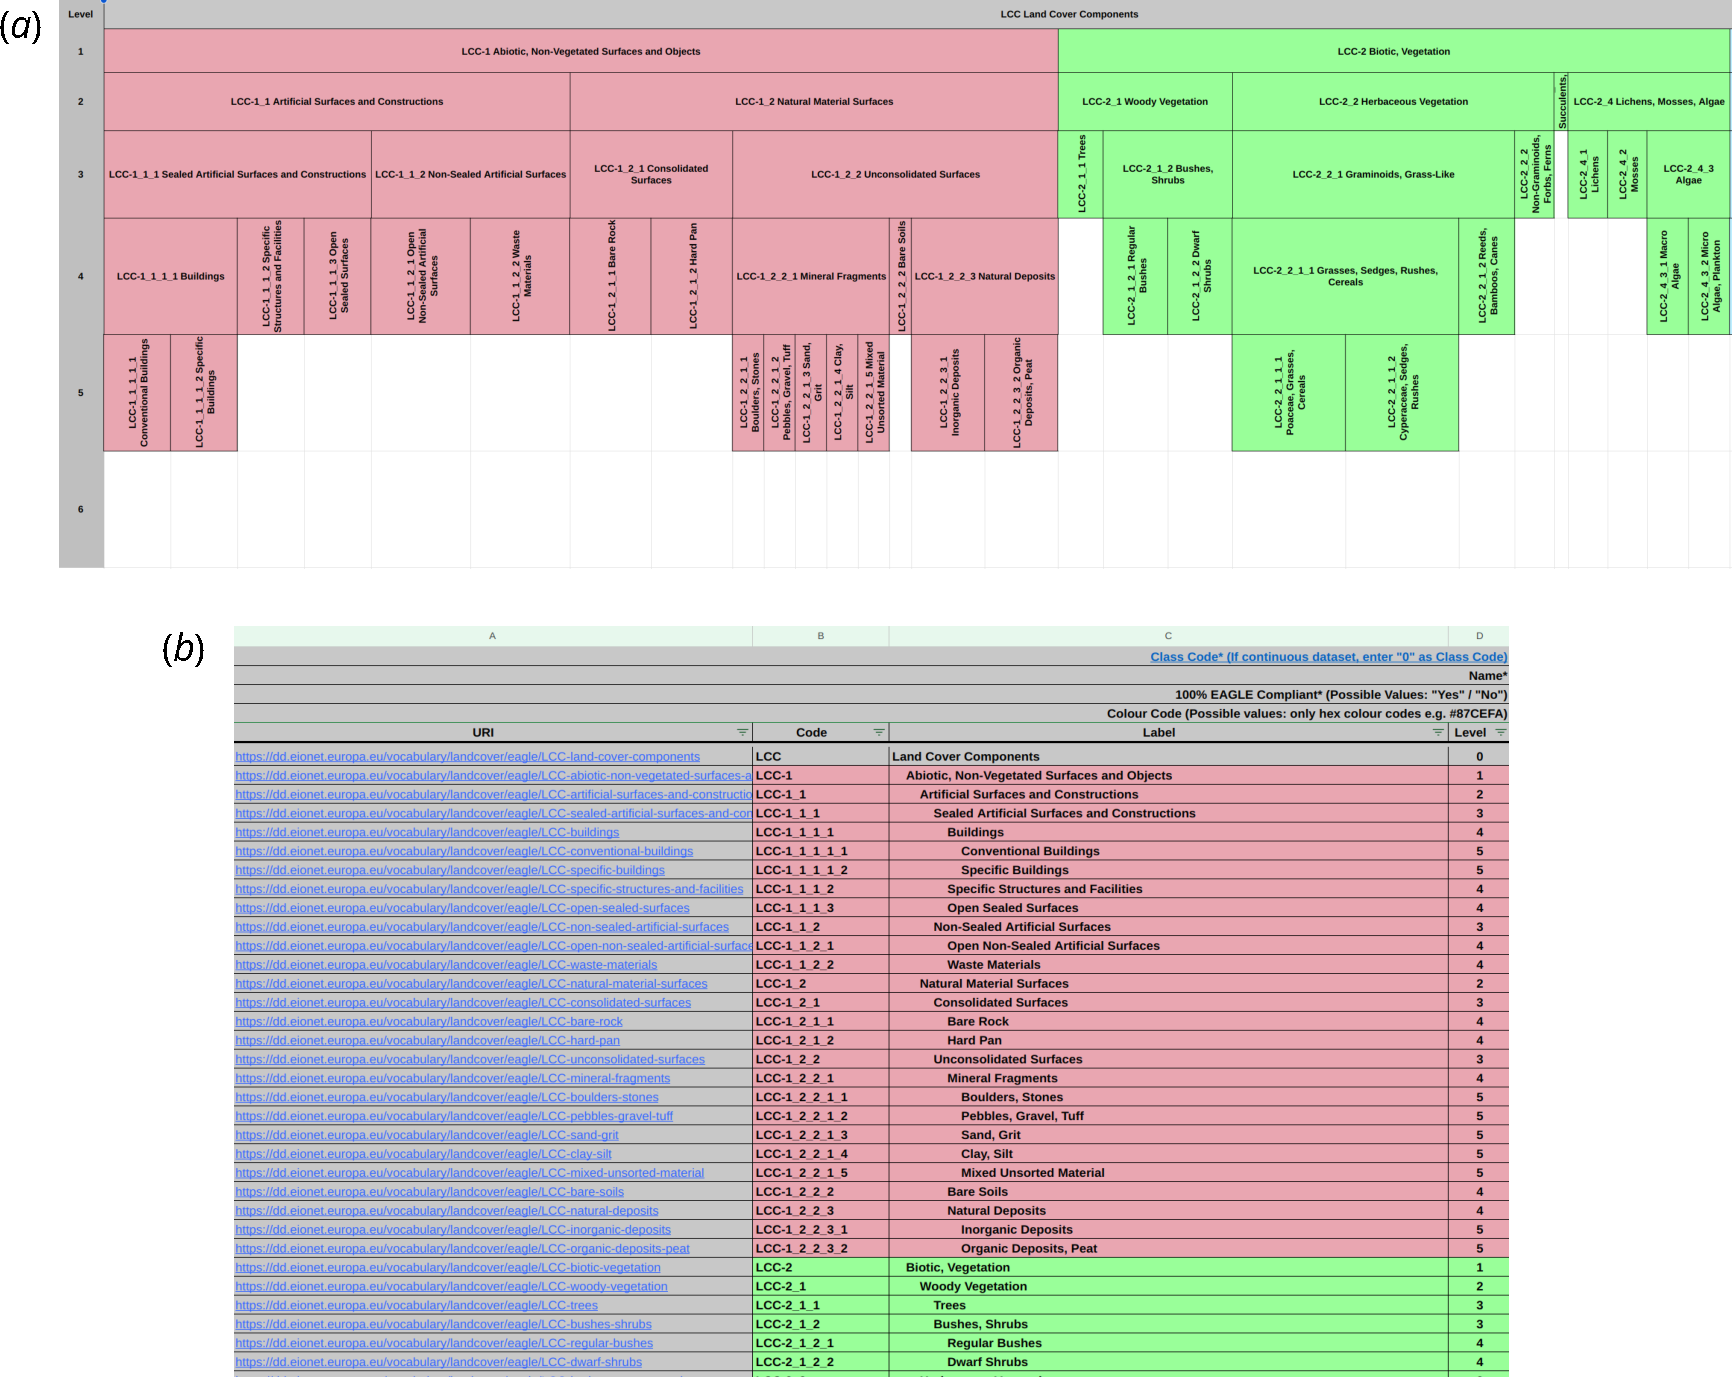
\includegraphics[width=\textwidth]{figs_01/fig_eagle_example.pdf}
%     \caption{EAGLE LCLU classification system preview.}
%     % https://land.copernicus.eu/en/eagle?tab=technical_implementation
%     \label{fig:01_xx}
% \end{figure}

% Many countries have their own classification systems (often in the local language), and these classification systems are often taken quite seriously by statistical offices and funding agencies, and tend to have more detailed and relevant legends higher quality than continental or global classification systems. For example, in the Netherlands... 

% The most comprehensive LCLU classification system to date is probably EAGLE. It is linked with a professional data dictionary, and every entry has a unique URL and is version-controlled. 

%     \subsection{Overview of existing continental and global scale land cover products}

%     Current publicly available global land cover and/or land use maps include (L. Liu et al. 2021):

% \begin{itemize}
%     \item GLASS-GLC is global land cover time-series 1982 to 2015 at 5-km resolution derived directly in Google Earth Engine (H. Liu et al. 2020).
%     \item MCD12Q1 Land Cover Type Yearly L3 Global product available in resolution from 500-km. MODIS Land cover maps (17 land cover classes based on the International Geosphere Biosphere Programme IGBP classification system) is a temporal dataset so that one can also derive various change indices and quantify the land cover dynamics.
%     \item ESA CCI Land cover is a global land cover time series from 1992 to 2020+ derived at 300-m spatial resolution from MERIS, SPOT and PROBA-V imagery. Maps can be accessed through a viewer and downloaded from the ESA website or from zenodo.org \citep{defourny2012land}.
%     \item Copernicus Global Land Cover products at 100-m for years 2015, 2016, 2017 and 2018 and based on the PROBA-V imagery \citep{buchhorn2020copernicus}. The maps can be downloaded directly from zenodo.org. These maps contain also predicted fractions for the main land cover classes.
%     \item GLAD Global Land Cover and Land Use Change 2000–2020 (GLCLUC2020) provides estimate of the land cover for the last 20+ years but also quantifies changes in forest extent and height, cropland, built-up lands, surface water, and perennial snow and ice extent (Potapov et al. 2022).
%     \item GLC FCS30D is a global 30-m annual land-cover time-series data set with 17-class system for the period 1982–2021 \citep{zhang2020glcfcs30}.
% \end{itemize}


% An in-depth review of time-series of global land cover / land use maps and their legends is also provided by \citet{mora2014global} and \citet{garcia2022global}.

% HYDE (History database of the Global Environment) contains historic (estimated) maps (10-km resolution) of main land use categories up to pre-historic times 10,000 BCE to CE 2020 (Klein Goldewijk et al. 2017). HYDE includes irrigated areas, rice, intensive pasture, extensive rangelands and similar. Data can be downloaded from the University of Utrecht Copernicus Land Change Lab.

% % glad https://glad.earthengine.app/view/glcluc-2000-2020#lon=4.795130882945959;lat=51.766156889096685;zoom=13;
% % cci https://openlandmap.org/?center=4.743565439381222,51.74520701831224&zoom=12.42439865444753&opacity=91&base=OpenStreetMap&layer=land.cover_esacci.lc.l4&time=2020
% % corine 

% A detailed Water mask of the world is available also from the Global Surface Water Explorer hosted by European Commission JRC \citep{pekel2016high}. A Landsat-based water dynamics assessment (annual maps) at 30-m is also provided by \citet{pickens2020mapping}. Global WaterPack (GWP) monthly and yearly product comprises different water coverage categories at 250-m spatial resolution.

% Due to the availability of the Sentinel-2 10~m resolution data, several land cover products are now available at very high resolution (but then only covering recent 3–5 years). These include:

% \begin{itemize}
%     \item Google Dynamic World at 10-m, limited to 9 classes but constantly updated (Brown et al. 2022);
%     \item ESA World Cover at 10-m based on Sentinel-1 and Sentinel-2 data for 2020 and 2021 available from Zenodo;
%     \item Global canopy top height map for the year 2020 at 10-m (Lang et al. 2023);
% \end{itemize}

% Several initiatives aim at integrating multiple land cover products \citep{herold2016toward}(Herold et al. 2016) and/or running land cover classification by fusing multisource EO data \citep{song2017improving,liu2021finer}.
% 

\subsection*{The current land cover mapping arms race}
        % https://viewer.esa-worldcover.org/worldcover/?language=en&bbox=4.469697541130503,51.68401389727245,4.9938756117307745,51.840819713845065&overlay=false&bgLayer=OSM&date=2024-03-13&layer=WORLDCOVER_2021_MAP
        
\begin{figure}[H]
    \centering
    \begin{subfigure}[b]{0.48\textwidth} % Adjusted to 0.48 to allow some space between images
        \centering
        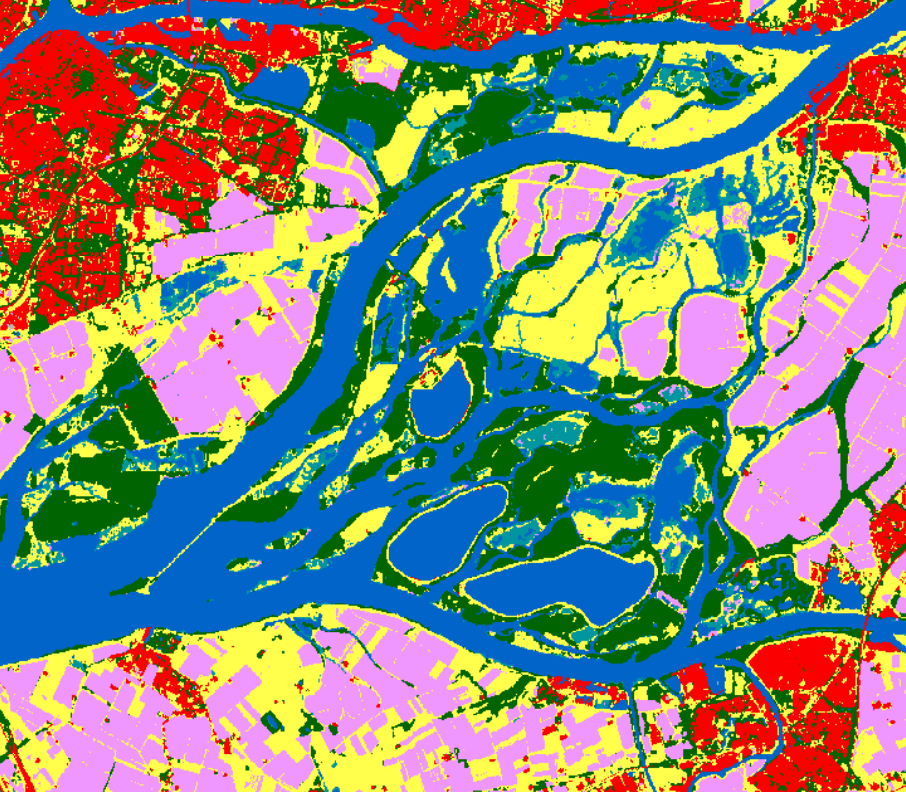
\includegraphics[width=0.99\textwidth,height=0.99\textwidth]{figs_01/a_worldcover.png}
        \caption{ESA WorldCover}
        \label{fig:lc_worldcover}
    \end{subfigure}
    \hfill % This adds a small horizontal space between the figures
    \begin{subfigure}[b]{0.48\textwidth} % Adjusted to 0.48 to allow some space between images
        \centering
        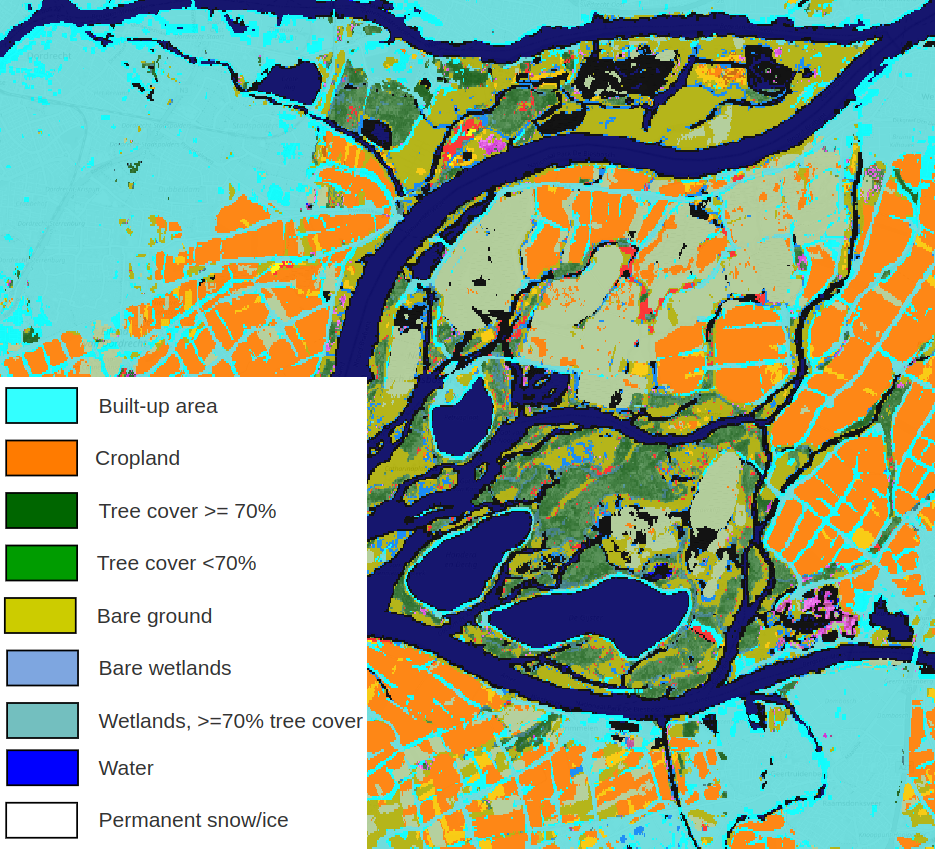
\includegraphics[width=0.99\textwidth,height=0.99\textwidth]{figs_01/a_glad.png}
        \caption{GLAD Land Cover}
        \label{fig:lc_glad}
    \end{subfigure}
    
    \vspace{1em} % This adds a bit of vertical space between the rows of figures

    \begin{subfigure}[b]{0.48\textwidth} % Adjusted to 0.48 to allow some space between images
        \centering
        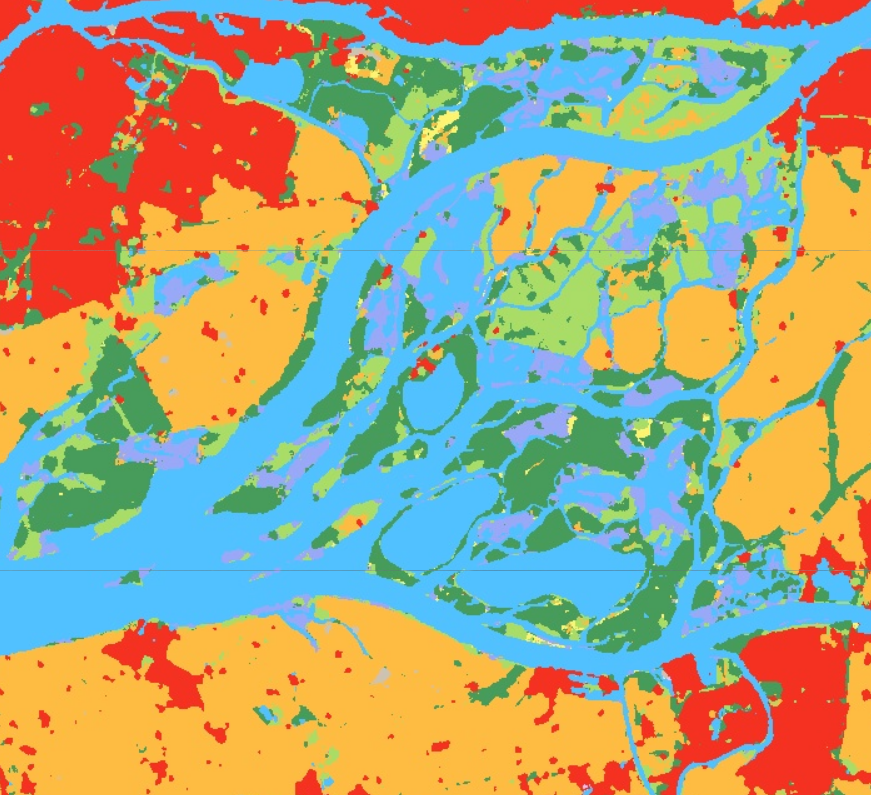
\includegraphics[width=0.99\textwidth,height=0.99\textwidth]{figs_01/a_dynamicworld.png}
        \caption{Google Dynamic World}
        \label{fig:lc_dynamicworld}
    \end{subfigure}
    \hfill % This adds a small horizontal space between the figures
    \begin{subfigure}[b]{0.48\textwidth} % Adjusted to 0.48 to allow some space between images
        \centering
        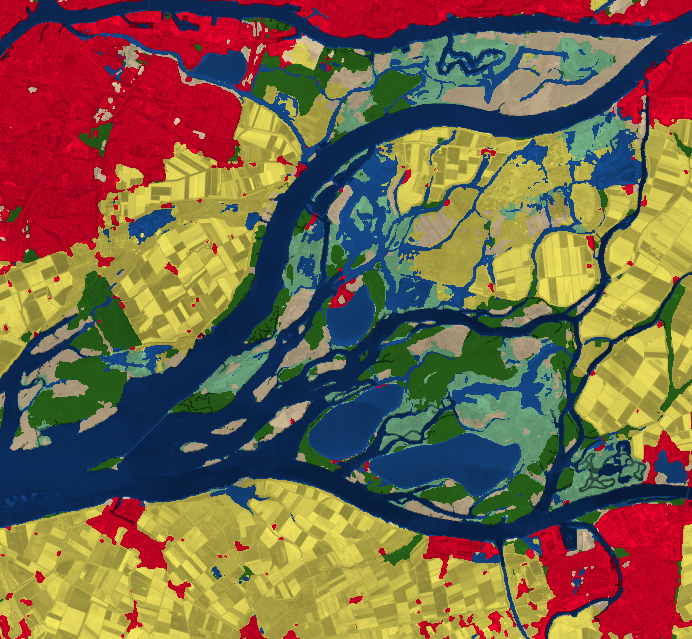
\includegraphics[width=0.99\textwidth,height=0.99\textwidth]{figs_01/a_esri.png}
        \caption{ESRI Land Cover}
        \label{fig:lc_esri}
    \end{subfigure}
    
    \caption{Example of four global mapping projects on the Biesbosch wetlands area in the Netherlands.}
    \label{fig:bigmaps_biesbosch}
\end{figure}
    
    In the last few years, several large-scale high-resolution land cover maps have been made at a global scale. Notable examples are ESA's WorldCover \citep{kerchove2021esa} and WorldCereal \citep{tricht2023worldcereal}, Google's DynamicWorld \citep{brown2022dynamic}, ESRI's Land Cover \citep{karra2021global}.
    These maps often have high resolution and high accuracy, but are usually limited in multiple ways: reproducibility, time coverage, and detail:
    
    \subsubsection{Reproducibility}
        The current big mapping initiatives only share their maps, not the reference data that they used to produce them. This not only makes it difficult or impossible to reproduce, validate \citep{venter2022global}, or improve their work, but also prevents it from being used for new projects \citep{tsendbazar2015assessing}.
    
    \subsubsection{Time coverage} 
        Most of the current generation of maps use 10~m Sentinel-2 data, which only became available in 2016. Mapping initiatives that use Landsat data can go back much further, but are then limited to mapping at 30m resolution. Examples are the Australian land cover time series made by \citep{calderon2021high} and the work of UMD GLAD, which produced annual land cover maps from the year 2000 onwards using Landsat data \citep{hansen2022global}.

    \subsubsection{Detail}
        %Visual interpretation mention specifically!
        Often, these maps depict at most ten land cover categories (see Table~\ref{tab:bigmaps}). Mapping more classes is more difficult because there is more chance of confusion between similar classes. This also applies to the creation of training data: The current most common way to create it is by visual inspection of high resolution aerial imagery, and this becomes more difficult with more specific classes. Just like for a machine learning model, it is much easier for an annotator to differentiate between a forest and cropland than between different cereal crop types. Classifying more different classes is also more difficult for machine learning models and requires more training data, and of higher quality, which is an expensive and complex task \citep{li2021improving}, especially for large diverse areas (e.g., continents or the whole planet) \citep{tsendbazar2021towards,stanimirova2023global}. 

    Although there are exceptions to each of these issues, in general, all mapping initiatives have at least one of these limitations (see Table\@~\ref{tab:bigmaps})

    \begin{table}[h]
    \centering
    \resizebox{\textwidth}{!}{%
    \begin{tabular}{|l|c|c|c|c|c}
    \hline
    \textbf{Mapping Product} & \textbf{Classes} & \textbf{Training Data} & \textbf{Validation Data} & \textbf{Time Extent}  \\ \hline
    ESA WorldCover \citep{zanaga2022esa}                    & 11    & No                                    & No                                    & two years \\ 
    \hline
    ESA WorldCereal \citep{tricht2023worldcereal}           &
    Google DynamicWorld \citep{brown2022dynamic}                                    & 9     & Yes \citep{tait2021dwtd}              & No                                    & 2016+, monthly \\ 
    \hline
    ESRI Land Cover \citep{karra2021global}                 & 9     & No                                    & No Information                        & One year () \\
    \hline
    \citep{zhang2020glc_fcs3}                               & 24    & ?                                     & ?                                     & Two years (2015,2020) \\
    \hline
    S2GLC Maps of Europe \citep{malinowski2020automated}    & 13    & No                                    & Yes \citep{jenerowicz2021validation}  & One year (2017) \\ 
    \hline
    ELC10 \citep{venter2021continentalscale}                & 8     & ?                                     & ?                                     & One year (2020) \\
    \hline
    Pan-European land cover \citep{pflugmacher2019mapping}  & 12    & Yes \citet{dandrimont2020harmonised}  & Yes (cross-validation)                & One year \\ 
    \hline
    Australian Land Cover \citep{calderon2021high}          & 6     & No                                    & No Information                        & 1985-2015 \\
    \end{tabular}
    }%
    \caption{Summary of Mapping Products and Data Availability}
    \label{tab:bigmaps}
    \end{table}

% However, the fact that there is now significant interest in getting the most current, most accurate, and most detailed (spatial resolution) products showing the dynamics of land cover and land use is excellent news! Fair competition should be embraced or as the famous Chinese poem says \emph{``Let a hundred flowers bloom; let a hundred schools of thought contend.''}

\section{Research Gaps}

    There is a reproducibility crisis in science, and environmental monitoring is no exception. How can decision-makers trust datasets whose creation does not only involve complex workflows, but can not be reproduced or improved? It turns out that they often don't, and keep relying on older methods that might be slow and expensive, but reproducible and reliable. The current boom in for-profit remote sensing has allowed for excellent analysis using high-resolution data ---e.g., drivers of deforestation in Africa \citep{masolele2024mapping} using 3~m resolution Planet data--- but limitations on sharing this data, and the profit and marketing motivations of corporations make sharing, trusting, and using their maps difficult.

    There are no large-scale maps with more than 13 classes, not even for Europe, for which an unprecedented wealth of land cover information is publicly available \citep{dandrimont2020harmonised}. \citet{pflugmacher2019mapping} demonstrated that the LUCAS points can be used to train and validate land cover models, but the LUCAS legend is a hierarchical system with over 70 land cover classes. To retain its use as a validation set, training data should be extracted from other human-annotated datasets such as CORINE, EuroCrops \citep{schneider2023eurocrops} and OpenStreetMap. In order to use data with the large minimal mapping unit of CORINE or the potential errors in volunteered geographical information \citep{neis2014recent}, filtering techniques are required to remove spurious training samples.

    Furthermore, while some long-term annual mapping projects exist, they either have a low spatial resolution like ESA CCI \citep{harper202229} or cover only a select set of classes \citep{hansen2022global}.

    Lastly, to evaluate the impacts of human activities on the environment and to both enable and justify localized interventions, it is essential that trends from area estimates and periodic maps are linked \citep{olofsson2014good,szantoi2020addressing,winkler2021global}. This requires a mapping framework that minimizes both quantity and allocation error \citep{pontius2011death}. While many mapping initiatives report class proportions \citep{pflugmacher2019mapping} or try to approximate correct area estimation with direct remote sensing measures \citep{kleinewillinghofer2022unbiased}, only a few explicitly investigate methods to force maps to match area estimates \citep{strahler1980use,horvath2021comparison}.
    

\section{Objectives}
\label{sec:research_objectives}
The overall objective of this PhD thesis is to take advantage of the availability of various open European land use / land cover datasets and statistics, and to combine these with Earth observation data and machine learning to make accurate, detailed maps that are compatible with the needs of European policy makers and researchers. More specifically, this thesis aims to answer the following research questions:

\begin{enumerate}
\item %The Value of Aggregating and Combining Time-Series and Static EO Data for Land Cover Classification: 
What are the benefits and challenges of combining multiple large time-series and static EO datasets into Analysis-Ready data for the purpose of land cover classification?
\item % The Value of a Spatiotemporal Approach for Land Cover Classification: 
To what extent does training data from multiple times and places improve the accuracy and generalization of land cover classification?
\item % The Effect of Legend Design and Size: 
How does the number and type of classes in a legend affect the accuracy of land cover classification?
\item % Ensuring Land Cover Maps Match Area Estimates Without Sacrificing Accuracy: 
What is the effect of enforcing correct class proportions on map accuracy?
\item % Obtaining Useful Prediction Uncertainty Estimates: 
Which uncertainty metric is most useful for optimizing the trade-off between detail and accuracy?
\end{enumerate}

\section{Thesis Outline}

The research questions posed in the previous section are answered through four research papers, which are presented as chapters in this thesis. Fig.\@~\ref{fig:01_rqs_chapters} provides a graphical overview of how each chapter relates to each research question framework. The first two chapters focus on combining earth observation and land cover data from multiple sources to train models that can generalize well to unknown years. The chapters 4 and 5 introduce and apply a novel algorithm that uses a-priori class proportions from area estimates to optimize the accuracy, quantity, and detail of predictions by such models.

\begin{figure}
    \centering
    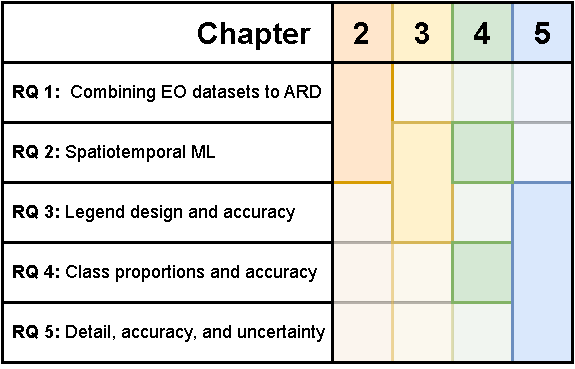
\includegraphics[width=\textwidth]{figs_01/fig_rqs_chapters.pdf}
    \caption{Overview of which chapters discuss which research questions}
    \label{fig:01_rqs_chapters}
\end{figure}


\textbf{Chapter 2} focuses on the benefits and challenges of harmonizing and combining large-scale spatiotemporal datasets for land cover mapping, most of which were used in the following chapters. The chapter details the work that went into creating, harmonizing, and imputing multiple Earth observation datasets (Landsat, Sentinel-2, and a new 30m resolution DTM) covering Europe. It introduces and describes the imputation algorithm TMWM that was used to impute the Landsat data, and validates its accuracy in a spatiotemporally explicit way. It then explores how combining the different datasets improves the accuracy of land cover classification models. Lastly, it shows that models trained on samples from a longer time range can generalize better to years that they have not been trained on.

\fullcite{witjes2023ecodatacube}

\textbf{Chapter 3} focuses on the production of annual land use / land cover maps of Europe for 2000-2020. It details the steps taken to harmonize and clean the training data from multiple openly available sources (CORINE, LUCAS) into a legend with 43 classes. A thorough accuracy assessment using cross-validation and an independent set of S2GLC validation points describes how well the model generalizes across space and time, and quantifies the trade-off imposed by having a legend with high thematic resolution. Results show that the maps have similar accuracy as other current continental-scale maps at low thematic resolution, and that a more detailed legend introduces more errors.

\fullcite{witjes2022spatiotemporal}

\textbf{Chapter 4} introduces IMP, an algorithm that uses land cover area estimates to iteratively classify land cover from existing probabilities, producing maps whose class proportions match the input estimates. It details the algorithm and showcases its use by mapping five European countries in five years. The accuracy of the maps is compared with maps created using highest likelihood classification. Results show that the proportional maps do not only have more accurate class proportions, but equal or better accuracy than highest likelihood maps. We also compare the accuracy and proportions of maps based on probabilities predicted by models trained on data representative of the area of interest, and probabilities predicted by a general model trained on large parts of Europe. Results show that maps based on general model predictions reach more accurate class proportions, while maps based on local model predictions are slightly more accurate. Finally, it presents an unintentional finding that the iterations at which the algorithm classifies certain pixels is related to the accuracy of those pixels, suggesting that it can be used to generate pixel-level accuracy estimates.

\fullcite{witjes2024iterative} 
(In review)

\textbf{Chapter 5} builds on the methods and findings of the previous chapters. 
Firstly, it presents a workflow to create larger and more detailed training datasets from multiple open data sources that are compatible with the hierarchical LUCAS land cover legend. 
Secondly, it investigates to what extent iteration classification uncertainty (ICU) can be used to provide reliable pixel-based uncertainty for land cover maps. It does this by creating high thematic resolution land cover maps of several NUTS2 regions across Europe, using Eurostat area estimates, training data extracted and harmonized from CORINE and EuroCrops, and validating them with LUCAS land cover points. 
The pixel-based error estimates are then used to aggregate uncertain predictions to more general classes and guarantee a baseline level of accuracy at the cost of some thematic detail. Different heuristics of prediction uncertainty are compared in their reliability to guarantee an error rate and the extent to which thematic detail must be sacrificed.

\fullcite{witjes2024hierarchical}
(Work in progress)